% <-- a percent symbol indicates a comment which does not affect the output of LaTeX
% you can leave the preamble alone, from here ...
\documentclass[12pt]{article}

\usepackage{amssymb,amsmath,amsthm}
\usepackage{tikz}
\usepackage[top=1in, bottom=1in, left=1.25in, right=1.25in]{geometry}
\usepackage{enumitem,palatino}
\usepackage{graphicx}
\usepackage[colorlinks=true,citecolor=blue,linkcolor=red,urlcolor=blue]{hyperref}

\newtheorem{problem}{Problem}
% ... to here

% shortcuts for blackboard bold number sets (reals, integers, etc.)
\newcommand{\II}{\ensuremath{\mathbb I}}
\newcommand{\NN}{\ensuremath{\mathbb N}}
\newcommand{\QQ}{\ensuremath{\mathbb Q}}
\newcommand{\RR}{\ensuremath{\mathbb R}}
\newcommand{\ZZ}{\ensuremath{\mathbb Z}}
\newcommand{\PP}{\ensuremath{\mathbb{P}}}

\newcommand{\eps}{\ensuremath{\epsilon}}
\newcommand{\ds}{\displaystyle}

% feel free to add more shortcuts here


\begin{document}
% replace with your name, but otherwise leave this header alone, from here ...
\small
\noindent \textsc{Math F307: Homework Assignment 4} \hfill Christopher Munoz

\normalsize
\bigskip
% ... to here

\section*{Section 3.1}

\setcounter{problem}{1}
\begin{problem}
Let $A = \{0, 1, 2\}$. Each of the statements below defines a relation $R$ on $A$ by $(m, n) \in R$ if the statement is true for $m$ and $n$. Write each of the relations as a set of ordered pairs.

\begin{enumerate}[label=(\alph*)]
    \item $m \leq n$
    
    \item $m < n$
    \setcounter{enumi}{5}
    
    \item $m + n \in A$
    \setcounter{enumi}{7}
    
    \item $m^2 + n^2 = 3$
\end{enumerate}
\end{problem}

\begin{proof}[Solution]
~
\begin{enumerate}[label=(\alph*)]
    \item $m \leq n$
    
    \textbf{Answer:} $R = \{(0, 0), (0, 1), (0, 2), (1, 1), (1, 2), (2, 2)\}$
    
    \item $m < n$
    
    \textbf{Answer:} $R = \{(0, 1), (0, 2), (1, 2)\}$
    
    \setcounter{enumi}{5}
    
    \item $m + n \in A$
        
    \textbf{Answer:} $R = \{(0, 0), (0, 1), (0, 2), (1, 0), (1, 1), (2, 0)\}$
    
    \setcounter{enumi}{7}
    
    \item $m^2 + n^2 = 3$

    \textbf{Answer:} $R = \emptyset$ (the empty set)
\end{enumerate}
\end{proof}

\setcounter{problem}{5}
\begin{problem}
Consider the relation $R$ on $\ZZ$ defined by $(m, n) \in R$ if and only if $m^3 - n^3 \equiv 0 \pmod{5}$. Which of the properties (R), (AR), (S), (AS), and (T) are satisfied by $R$?

Note: (R) = Reflexive, (AR) = Antireflexive, (S) = Symmetric, (AS) = Antisymmetric, (T) = Transitive
\end{problem}

\begin{proof}[Solution]
  R is reflexive, symmetric and transitive making R an equivalence relation. In fact module n partitions the integers into equivalence classes.
\end{proof}

\newpage

\setcounter{problem}{6}
\begin{problem}
Define the "divides" relation $R$ on $\NN$ by $(m, n) \in R$ if $m \mid n$.

\begin{enumerate}[label=(\alph*)]
    \item Which of the properties (R), (AR), (S), (AS), and (T) does $R$ satisfy?
\end{enumerate}
\end{problem}

\begin{proof}[Solution]

  $R$ satisfies reflexivity and transitivity but does not satisfy symmetry making it anti-symmetric, thus it is a partial order.
\end{proof}


\setcounter{problem}{9}
\begin{problem}
Give an example of a relation that is:

\begin{enumerate}[label=(\alph*)]
    \item antisymmetric and transitive but not reflexive,
    
    \item symmetric but not reflexive or transitive.
\end{enumerate}

\end{problem}

\begin{proof}[Solution]
~
\begin{enumerate}[label=(\alph*)]
    \item \textbf{Antisymmetric and transitive but not reflexive:}
    
   The greater than relation $>$ on $\RR$ (or on any set of numbers).
    
    Define $R$ on $\RR$ by: $(a, b) \in R$ if and only if $a > b$.
    
    \textbf{Not Reflexive:} For any $a \in \RR$, we have $a \not> a$, so $(a, a) \notin R$.
    
    \textbf{Antisymmetric:} If $(a, b) \in R$ and $(b, a) \in R$, then $a > b$ and $b > a$, which is impossible. So vacuously, the implication holds (antisymmetric).
     
    \textbf{Transitive:} If $a > b$ and $b > c$, then $a > c$ by the transitivity of $>$. So $(a, b) \in R$ and $(b, c) \in R$ implies $(a, c) \in R$.   
    \item \textbf{Symmetric but not reflexive or transitive:}
    
    Let $S = \{1, 2, 3\}$ and $R = \{(1, 2), (2, 1), (2, 3), (3, 2)\}$.
    
    \textbf{Not Reflexive:} $(1, 1) \notin R$, $(2, 2) \notin R$, $(3, 3) \notin R$.
    
    \textbf{Symmetric:} $(1, 2) \in R$ and $(2, 1) \in R$ $\checkmark$. $(2, 3) \in R$ and $(3, 2) \in R$ $\checkmark$.
    
    \textbf{Not Transitive:} $(1, 2) \in R$ and $(2, 3) \in R$, but $(1, 3) \notin R$.
    
    \begin{center}
    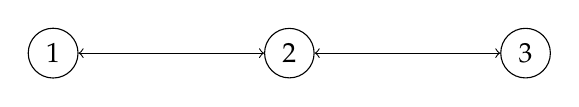
\begin{tikzpicture}[scale=1.5]
    \node[circle,draw] (1) at (0,0) {1};
    \node[circle,draw] (2) at (2,0) {2};
    \node[circle,draw] (3) at (4,0) {3};
    
    \draw[<->] (1) -- (2);
    \draw[<->] (2) -- (3);
    \end{tikzpicture}
    \end{center}
\end{enumerate}
\end{proof}

\newpage

\setcounter{problem}{17}
\begin{problem}
Draw pictures of each of the relations in Exercise 2 for parts (a), (b), (f), and (h). Use double-headed arrows or two arrows when the relation is symmetric.

From Exercise 2 on $A = \{0, 1, 2\}$:

(a) $m \leq n$: $R = \{(0, 0), (0, 1), (0, 2), (1, 1), (1, 2), (2, 2)\}$

(b) $m < n$: $R = \{(0, 1), (0, 2), (1, 2)\}$

(f) $m + n \in A$: $R = \{(0, 0), (0, 1), (0, 2), (1, 0), (1, 1), (2, 0)\}$

(h) $m^2 + n^2 = 3$: $R = \emptyset$
\end{problem}

\begin{proof}[Solution]
~

\textbf{(a) $m \leq n$:} NOT symmetric (e.g., $(0, 1) \in R$ but $(1, 0) \notin R$).

\begin{center}
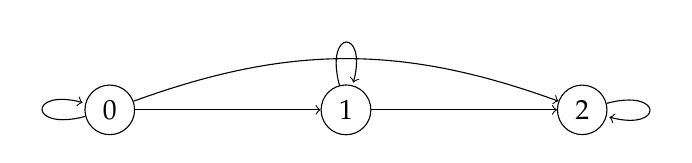
\begin{tikzpicture}[scale=1.5]
\node[circle,draw] (0) at (0,0) {0};
\node[circle,draw] (1) at (2,0) {1};
\node[circle,draw] (2) at (4,0) {2};

\draw[->] (0) edge[loop left] (0);
\draw[->] (1) edge[loop above] (1);
\draw[->] (2) edge[loop right] (2);
\draw[->] (0) -- (1);
\draw[->,bend left=20] (0) to (2);
\draw[->] (1) -- (2);
\end{tikzpicture}
\end{center}

\vspace{0.3in}

\textbf{(b) $m < n$:} NOT symmetric.

\begin{center}
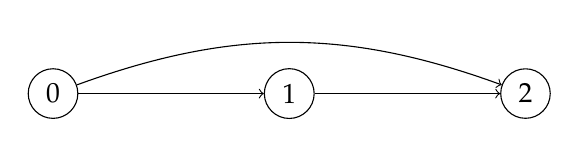
\begin{tikzpicture}[scale=1.5]
\node[circle,draw] (0) at (0,0) {0};
\node[circle,draw] (1) at (2,0) {1};
\node[circle,draw] (2) at (4,0) {2};

\draw[->] (0) -- (1);
\draw[->,bend left=20] (0) to (2);
\draw[->] (1) -- (2);
\end{tikzpicture}
\end{center}

\vspace{0.3in}

\textbf{(f) $m + n \in A$:} IS symmetric: $(0, 1)$ and $(1, 0)$ both in $R$; $(0, 2)$ and $(2, 0)$ both in $R$.

\begin{center}
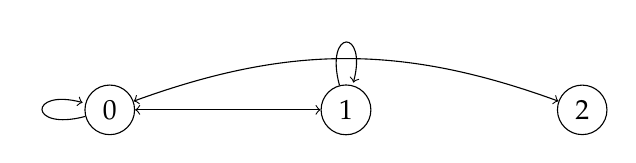
\begin{tikzpicture}[scale=1.5]
\node[circle,draw] (0) at (0,0) {0};
\node[circle,draw] (1) at (2,0) {1};
\node[circle,draw] (2) at (4,0) {2};

\draw (0) edge[loop left] (0);
\draw (1) edge[loop above] (1);
\draw[<->] (0) -- (1);
\draw[<->,bend left=20] (0) to (2);
\end{tikzpicture}
\end{center}

\vspace{0.3in}

\textbf{(h) $m^2 + n^2 = 3$:} Empty relation, no edges.

\begin{center}
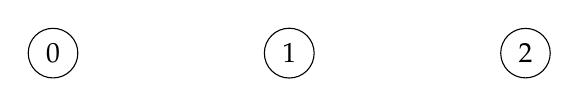
\begin{tikzpicture}[scale=1.5]
\node[circle,draw] (0) at (0,0) {0};
\node[circle,draw] (1) at (2,0) {1};
\node[circle,draw] (2) at (4,0) {2};
\end{tikzpicture}
\end{center}

\end{proof}

\newpage

\section*{Section 3.2}

\setcounter{problem}{1}
\begin{problem}
Draw a picture of the digraph $G$ with vertex set $V(G) = \{w, x, y, z\}$, edge set $E(G) = \{a, b, c, d, e, f, g\}$, and $\gamma$ given by:

\begin{center}
\begin{tabular}{|c|c|c|c|c|c|c|c|}
\hline
$e$ & $a$ & $b$ & $c$ & $d$ & $e$ & $f$ & $g$ \\
\hline
$\gamma(e)$ & $(x, w)$ & $(w, x)$ & $(x, x)$ & $(w, z)$ & $(w, y)$ & $(w, z)$ & $(z, y)$ \\
\hline
\end{tabular}
\end{center}
\end{problem}

\begin{proof}[Solution]
~

The digraph has edges:
\begin{itemize}
    \item Edge $a$: $x \to w$
    \item Edge $b$: $w \to x$
    \item Edge $c$: $x \to x$ (loop)
    \item Edge $d$: $w \to z$
    \item Edge $e$: $w \to y$
    \item Edge $f$: $w \to z$ (parallel to $d$)
    \item Edge $g$: $z \to y$
\end{itemize}

\begin{center}
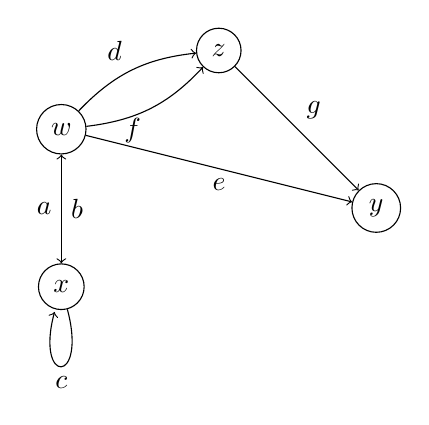
\begin{tikzpicture}[scale=2]
\node[circle,draw] (w) at (0,1) {$w$};
\node[circle,draw] (x) at (0,0) {$x$};
\node[circle,draw] (y) at (2,0.5) {$y$};
\node[circle,draw] (z) at (1,1.5) {$z$};

\draw[->] (x) -- node[left] {$a$} (w);
\draw[->] (w) -- node[right] {$b$} (x);
\draw[->] (x) edge[loop below] node[below] {$c$} (x);
\draw[->,bend left=20] (w) to node[above left] {$d$} (z);
\draw[->,bend right=20] (w) to node[below left] {$f$} (z);
\draw[->] (w) -- node[below] {$e$} (y);
\draw[->] (z) -- node[above right] {$g$} (y);
\end{tikzpicture}
\end{center}

\end{proof}

\newpage

\setcounter{problem}{2}
\begin{problem}
Which of the following vertex sequences describe paths in the digraph pictured in Figure 7(a)?

\begin{enumerate}[label=(\alph*)]
    \item $z\ y\ v\ w\ t$
    \item $x\ z\ w\ t$
    \item $v\ s\ t\ x$
    \item $z\ y\ s\ u$
    \item $x\ z\ y\ v\ s$
    \item $s\ u\ x\ t$
\end{enumerate}

\begin{center}
\includegraphics[width=0.8\textwidth]{figures32/Figure7.png}
\end{center}
\end{problem}

\begin{proof}[Solution]
Below we checkmark the valid paths and x mark the invalid ones:
\begin{enumerate}[label=(\alph*)]
    \item $z\ y\ v\ w\ t \checkmark$
    \item $x\ z\ w\ t \checkmark$
    \item $v\ s\ t\ x \times$
    \item $z\ y\ s\ u \times$
    \item $x\ z\ y\ v\ s \checkmark$
    \item $s\ u\ x\ t \times$
\end{enumerate}

\end{proof}

\newpage

\setcounter{problem}{4}
\begin{problem}
Consider the digraph pictured in Figure 7(b). Describe an acyclic path

\begin{enumerate}[label=(\alph*)]
    \item from $x$ to $y$
    \setcounter{enumi}{4}
    
    \item from $z$ to $v$
\end{enumerate}
\end{problem}

\begin{proof}[Solution]
    \item from $x$ to $y$ : x w y
    \setcounter{enumi}{4}
    
    \item from $z$ to $v$ : z y v
\end{proof}



\setcounter{problem}{5}
\begin{problem}
There are four basic blood types: A, B, AB, and O. Type O can donate to any of the four types, A and B can donate to AB as well as to their own types, but type AB can only donate to AB. Draw a digraph that presents this information. Is the digraph acyclic?
\end{problem}

\begin{proof}[Solution]
~

Vertices: $\{O, A, B, AB\}$
\begin{center}
\begin{tikzpicture}[scale=1.8]
\node[circle,draw] (O) at (0,2) {O};
\node[circle,draw] (A) at (2,3) {A};
\node[circle,draw] (B) at (2,1) {B};
\node[circle,draw] (AB) at (4,2) {AB};

\draw[->] (O) edge[loop left] (O);
\draw[->,bend left=15] (O) to (A);
\draw[->,bend right=15] (O) to (B);
\draw[->] (O) to (AB);

\draw[->] (A) edge[loop above] (A);
\draw[->,bend left=15] (A) to (AB);

\draw[->] (B) edge[loop below] (B);
\draw[->,bend right=15] (B) to (AB);

\draw[->] (AB) edge[loop right] (AB);
\end{tikzpicture}
\end{center}

Graph is not acyclic, Each vertex has a self-loop (cycle of length 1).

\end{proof}

\newpage

\setcounter{problem}{7}
\begin{problem}
Determine the reachability relation for the digraphs in Figures 6(a), (c), and (d).

\begin{center}
\includegraphics[width=0.8\textwidth]{figures32/Figure6.png}
\end{center}
\end{problem}

\begin{proof}[Solution]
~
\begin{align*}
  R(a) &= \{(v,w),(v,y),(v,x),(v,v),(w,y),(w,x),(w,v), \\ 
   &\quad (w,w)(y,x),(y,v),(y,w),(y,y),(x,v),(x,w),(x,y),(x,x)\} \\ \\
    R(c) &= \{(w,x),(x,w),(y,z),(z,y),(w,w),(x,x),(y,y),(z,z)\} \\ \\
  R(d) &= \{(x,x),(y,y),(z,z),(x,y),(x,z),(y,z)\}
\end{align*}


\end{proof}

\newpage

\setcounter{problem}{14}
\begin{problem}
Give the adjacency relation $A$ and the reachable relation $R$ for each of the graphs of Figure 8.

\begin{center}
\includegraphics[width=0.8\textwidth]{figures32/Figure8.png}
\end{center}
\end{problem}

\begin{proof}[Solution]
\begin{align*}
  A(a) &= \{(y,y),(w,w),(y,w),(w,y),(w,x),(x,w),(x,z),(z,x)\} \\
  R(a) &= \{(y,y),(w,w),(x,x),(z,z),(y,w),(y,x),(y,z),(w,y),(w,x),(w,z)\\
       &\quad (x,w),(x,y),(x,z),(z,x),(z,w),(z,y)\} \\ \\
    A(b) &= \{(y,v)(v,w),(w,w),(w,v),(v,y),(z,z)\} \\
    R(b) &= \{(y,y),(v,v),(w,w),(y,v),(y,w), (v,y),(v,w),(w,v),(w,y),(z,z)\}
\end{align*}

\end{proof}

\setcounter{problem}{15}
\begin{problem}
For the graph in Figure 8(a), give an example of each of the following. Be sure to specify the edge sequence and the vertex sequence.

\begin{enumerate}[label=(\alph*)]
    \item a path of length 2 from $w$ to $z$.
    
    \item a path of length 4 from $z$ to itself.
    
    \item a path of length 5 from $z$ to itself.
    
    \item a path of length 3 from $w$ to $x$.
\end{enumerate}
\end{problem}

\begin{proof}[Solution]
\begin{align*}
  (a) &\quad V(a) = (w,z), (x,z) &&\quad E(a) = d,f \\
  (b) &\quad V(b) = (z,x),(x,z),(z,x),(x,z) &&\quad E(b) = g, e, f, g \\
  (c) &\quad V(c) = (z,x),(x,w),(w,w),(w,x),(x,z) &&\quad E(c) = f,d,a,d,f \\
  (d) &\quad V(d) = (w,w),(w,w),(w,x) &&\quad E(d) = a,a,d
\end{align*}

\end{proof}

\newpage

\section*{Section 3.3}

\setcounter{problem}{14}
\begin{problem}
Give the matrices for the digraphs in Figure 3.

\begin{center}
\includegraphics[width=0.7\textwidth]{figures33/figure3.png}
\end{center}
\end{problem}

\begin{proof}[Solution]
~
\begin{align*} 
  (a) = 
\begin{bmatrix}
  0 & 0 & 1 & 0 \\
  0 & 0 & 1 & 0 \\
  0 & 0 & 0 & 0 \\
  0 & 0 & 1 & 0
\end{bmatrix}
  (b) =
 \begin{bmatrix}
  1 & 1 & 0 & 0 \\
  1 & 1 & 0 & 2 \\
  0 & 0 & 0 & 2 \\
  0 & 0 & 0 & 0
\end{bmatrix}
  (c) =
 \begin{bmatrix}
  0 & 0 & 0 & 0 \\
  0 & 0 & 0 & 2 \\
  0 & 0 & 1 & 0 \\
  0 & 1 & 0 & 0
\end{bmatrix}
\end{align*}


\end{proof}

\newpage

\setcounter{problem}{15}
\begin{problem}
Write matrices for the graphs in Figure 4.

\begin{enumerate}[label=(\alph*)]
    \setcounter{enumi}{2}
    \item (Figure 4(c))
    
    \item (Figure 4(d))
\end{enumerate}

\begin{center}
\includegraphics[width=0.7\textwidth]{figures33/figure4.png}
\end{center}
\end{problem}

\begin{proof}[Solution]
~
\begin{align*} 
  (c) = 
\begin{bmatrix}
  0 & 1 & 1 & 0 & 0\\
  1 & 0 & 0 & 1 & 1\\
  1 & 0 & 0 & 1 & 1\\
  0 & 1 & 1 & 0 & 1 \\
  0 & 1 & 1 & 1 & 0
\end{bmatrix}
  (d) =
 \begin{bmatrix}
  0 & 1 & 0 & 0 \\
  1 & 1 & 0 & 0 \\
  0 & 0 & 1 & 0 \\
  0 & 0 & 0 & 0
\end{bmatrix}
\end{align*}


\end{proof}

\newpage

\setcounter{problem}{16}
\begin{problem}
For each matrix in Figure 5, draw a digraph having the matrix.

\begin{enumerate}[label=(\alph*)]
    \setcounter{enumi}{1}
    \item (Matrix from Figure 5(b))
    
    \item (Matrix from Figure 5(c))
\end{enumerate}

\begin{center}
\includegraphics[width=0.7\textwidth]{figures33/figure5.png}
\end{center}
\end{problem}

\begin{proof}[Solution]
~
(b)
% First matrix: 1 1 0 1 / 0 3 0 2 / 0 0 0 0 / 2 0 0 1
\begin{center}
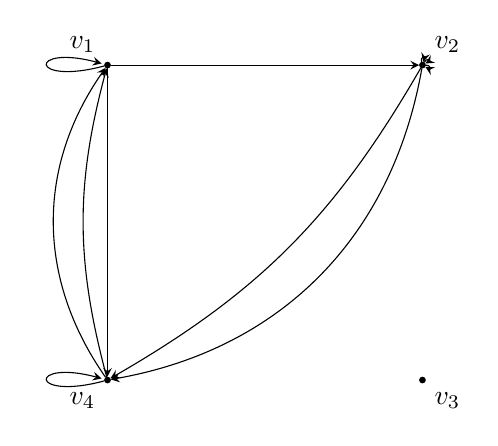
\begin{tikzpicture}[scale=2,
    vertex/.style={circle,draw,fill=black,minimum size=2pt,inner sep=0pt},
    >=stealth]

\node[vertex,label=above left:$v_1$] (v1) at (0,2) {};
\node[vertex,label=above right:$v_2$] (v2) at (2,2) {};
\node[vertex,label=below right:$v_3$] (v3) at (2,0) {};
\node[vertex,label=below left:$v_4$] (v4) at (0,0) {};

% From v1: loop, to v2, to v4
\draw[->] (v1) edge[loop left] (v1);
\draw[->] (v1) -- (v2);
\draw[->] (v1) -- (v4);

% From v2: 3 loops, 2 edges to v4
\draw[->] (v2) edge[loop above,looseness=8] (v2);
\draw[->] (v2) edge[loop right,looseness=8,in=30,out=60] (v2);
\draw[->] (v2) edge[loop right,looseness=8,in=-30,out=0] (v2);
\draw[->,bend left=15] (v2) to (v4);
\draw[->,bend left=35] (v2) to (v4);

% From v3: nothing

% From v4: 2 edges to v1, 1 loop
\draw[->,bend left=15] (v4) to (v1);
\draw[->,bend left=35] (v4) to (v1);
\draw[->] (v4) edge[loop left] (v4);

\end{tikzpicture}
\end{center}

(c)
% Second matrix: 0 1 0 0 0 / 0 0 1 0 0 / 0 0 0 1 0 / 0 0 0 0 1 / 1 0 0 0 0
\begin{center}
\begin{tikzpicture}[scale=1.5,
    vertex/.style={circle,draw,fill=black,minimum size=2pt,inner sep=0pt},
    >=stealth]

% Pentagon arrangement
\node[vertex,label=above:$v_1$] (v1) at (90:2) {};
\node[vertex,label=above right:$v_2$] (v2) at (18:2) {};
\node[vertex,label=below right:$v_3$] (v3) at (-54:2) {};
\node[vertex,label=below left:$v_4$] (v4) at (-126:2) {};
\node[vertex,label=above left:$v_5$] (v5) at (162:2) {};

% Cycle: v1->v2->v3->v4->v5->v1
\draw[->] (v1) to[bend left=15] (v2);
\draw[->] (v2) to[bend left=15] (v3);
\draw[->] (v3) to[bend left=15] (v4);
\draw[->] (v4) to[bend left=15] (v5);
\draw[->] (v5) to[bend left=15] (v1);

\end{tikzpicture}
\end{center}

\end{proof}

\newpage

\setcounter{problem}{17}
\begin{problem}
For each matrix in Figure 6, draw a graph having the matrix.

\begin{enumerate}[label=(\alph*)]
    \setcounter{enumi}{2}
    \item (Matrix from Figure 6(c)
    
    \item (Matrix from Figure 6(d))
\end{enumerate}

\begin{center}
\includegraphics[width=0.7\textwidth]{figures33/figure6.png}
\end{center}
\end{problem}

\begin{proof}[Solution]
  (c)
% First matrix: 0 2 1 0 / 2 0 0 1 / 1 0 1 0 / 0 1 0 1
\begin{center}
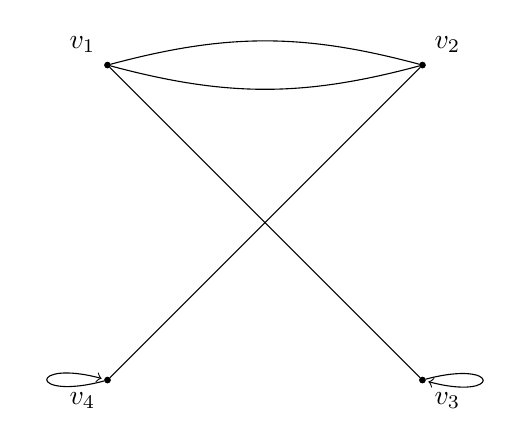
\begin{tikzpicture}[scale=2,
    vertex/.style={circle,draw,fill=black,minimum size=2pt,inner sep=0pt}]

\node[vertex,label=above left:$v_1$] (v1) at (0,2) {};
\node[vertex,label=above right:$v_2$] (v2) at (2,2) {};
\node[vertex,label=below right:$v_3$] (v3) at (2,0) {};
\node[vertex,label=below left:$v_4$] (v4) at (0,0) {};

% v1-v2: 2 parallel edges
\draw (v1) to[bend left=15] (v2);
\draw (v1) to[bend right=15] (v2);

% v1-v3: 1 edge
\draw (v1) -- (v3);

% v2-v4: 1 edge
\draw (v2) -- (v4);

% v3: 1 loop
\draw (v3) edge[loop right] (v3);

% v4: 1 loop
\draw (v4) edge[loop left] (v4);

\end{tikzpicture}
\end{center}
(d) (Trust me, there are two loops  for v1 and v2, just tiny)
% Second matrix: 2 0 0 0 0 / 0 2 0 0 0 / 0 0 1 0 0 / 0 0 0 0 1 / 0 0 0 1 0
\begin{center}
\begin{tikzpicture}[scale=1.5,
    vertex/.style={circle,draw,fill=black,minimum size=2pt,inner sep=0pt}]

% Arrange vertices in a line
\node[vertex,label=above:$v_1$] (v1) at (0,0) {};
\node[vertex,label=above:$v_2$] (v2) at (1.5,0) {};
\node[vertex,label=above:$v_3$] (v3) at (3,0) {};
\node[vertex,label=above:$v_4$] (v4) at (4.5,0) {};
\node[vertex,label=above:$v_5$] (v5) at (6,0) {};

% v1: 2 loops
\draw (v1) edge[loop left,looseness=8] (v1);
\draw (v1) edge[loop above,looseness=8] (v1);

% v2: 2 loops
\draw (v2) edge[loop left,looseness=8,in=100,out=140] (v2);
\draw (v2) edge[loop above,looseness=8,in=40,out=80] (v2);

% v3: 1 loop
\draw (v3) edge[loop above] (v3);

% v4-v5: 1 edge
\draw (v4) -- (v5);

\end{tikzpicture}
\end{center}

\end{proof}

\end{document}
